% Preview of every GEMMA figure and table at ACM sigconf geometry (7.0in text, 3.33in columns).
% xelatex preview.tex   (the real paper uses acmart; copy the figure/table blocks and captions from here)
\documentclass[9pt,twocolumn]{extarticle}
\usepackage[paperwidth=8.5in,paperheight=11in,textwidth=7in,textheight=9.25in,columnsep=0.33in,top=0.85in]{geometry}
\usepackage{fontspec}\usepackage{unicode-math}
\setmainfont{LibertinusSerif}[Path=../fonts/, Extension=.otf, UprightFont=*-Regular, ItalicFont=*-Italic, BoldFont=*-Bold]
\setsansfont{LibertinusSans}[Path=../fonts/, Extension=.otf, UprightFont=*-Regular, ItalicFont=*-Italic, BoldFont=*-Bold]
\setmathfont{LibertinusMath-Regular.otf}[Path=../fonts/]
\usepackage{graphicx,booktabs,multirow}
\usepackage[table]{xcolor}
\usepackage[font=small,labelfont=bf]{caption}
\definecolor{gemmarow}{HTML}{FDF0EA}
\AtBeginDocument{\renewcommand{\checkmark}{\mbox{\fontspec{DejaVu Sans}\char"2713}}}
\graphicspath{{../out/figs/}{../arch/}}
\newcommand{\gemma}{\textsc{Gemma}}
\begin{document}
\section*{GEMMA -- figures and tables (preview)}

% ---------------------------------------------------------------- Figure 1
\begin{figure*}[t]
\centering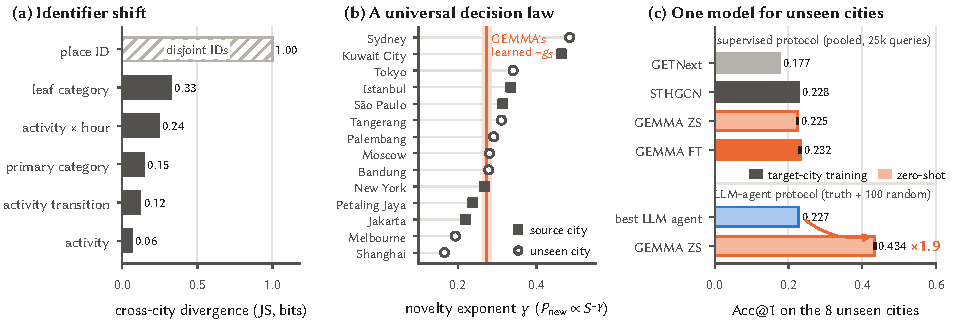
\includegraphics[width=\textwidth]{fig1_teaser.pdf}
\caption{\textbf{What transfers across cities.} (a)~Place identifiers are disjoint between cities (cross-city
Jensen--Shannon divergence $=1$ bit); the more abstract the description of a visit, the more cities share it.
(b)~The novelty exponent $\gamma$ of the exploration law $P(\text{new})\propto S^{-\gamma}$ in the 14 evaluated cities; the
orange band is the gate coefficient $-g_S$ that \gemma{} learns on the six source cities without ever being given
$\gamma$. (c)~Accuracy on the eight cities \gemma{} never saw: zero-shot \gemma{} is within 0.3 points of STHGCN,
which is trained in each city, and nearly doubles the best LLM agent; light fine-tuning on the training split
exceeds STHGCN.}
\label{fig:teaser}
\end{figure*}

% ---------------------------------------------------------------- Figure 2
\begin{figure*}[t]
\centering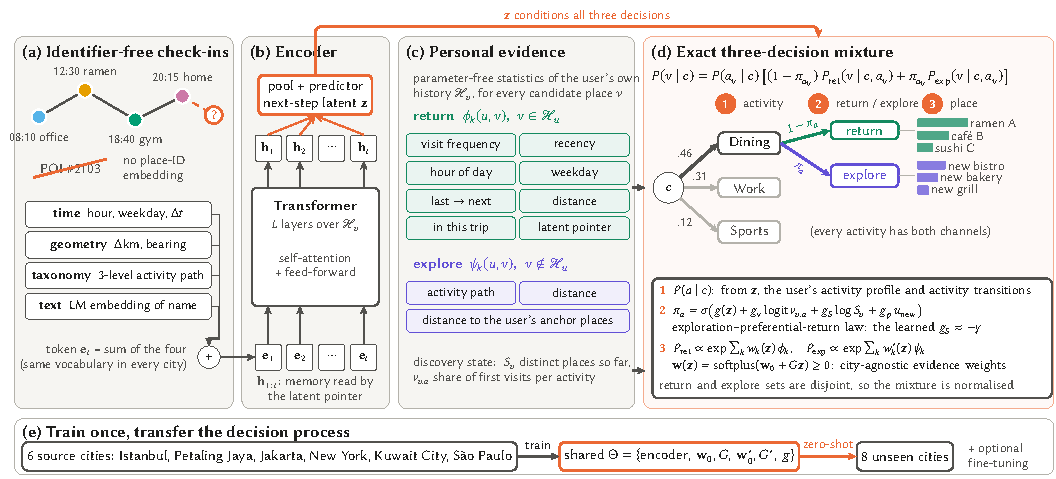
\includegraphics[width=\textwidth]{gemma_arch.pdf}
\caption{\textbf{\gemma.} (a)~Check-ins are tokens built from time, relative geometry, the activity taxonomy and a
language embedding of the place, never from a place identifier. (b)~A Transformer encodes the user's history into
states $\mathbf{h}_{1:t}$ and a next-step latent $\mathbf{z}$. (c)~Parameter-free statistics of the user's own
history score every candidate place. (d)~The next-place distribution factorises exactly into three decisions: the
activity, a gate between returning and exploring that follows the exploration--preferential-return law, and the
place, scored by non-negative, context-modulated evidence weights. (e)~All parameters act on statistics, so the
model trained on six cities is applied unchanged to unseen cities.}
\label{fig:arch}
\end{figure*}

\begin{table}[t]
\caption{Massive-STEPS cities. \emph{Queries}: test next-visit queries kept by the STHGCN protocol (target POI and user
seen in training). \emph{Revisit}: share of check-ins to an already visited place, over all check-ins and over the
scored queries. $\gamma$: novelty exponent of $P(\text{new})\propto S^{-\gamma}$.}
\label{tab:datasets}
\small\setlength{\tabcolsep}{3.2pt}
\begin{tabular}{lrrrrccc}
\toprule
City & Users & Check-ins & POIs & Queries & \multicolumn{2}{c}{Revisit} & $\gamma$ \\
 & & & & & all & test & \\
\midrule
\multicolumn{8}{l}{\textit{Source (training)}} \\
Istanbul & 23,700 & 544,471 & 42,795 & 41,150 & 0.40 & 0.50 & 0.33 \\
Petaling Jaya & 14,308 & 506,430 & 53,650 & 33,889 & 0.37 & 0.44 & 0.24 \\
Jakarta & 8,336 & 412,100 & 71,150 & 24,402 & 0.41 & 0.53 & 0.22 \\
New York & 6,929 & 272,368 & 45,804 & 16,766 & 0.37 & 0.45 & 0.27 \\
Kuwait City & 9,628 & 232,706 & 13,455 & 17,753 & 0.45 & 0.56 & 0.46 \\
São Paulo & 5,822 & 256,824 & 34,881 & 16,523 & 0.51 & 0.62 & 0.31 \\
\midrule
\multicolumn{8}{l}{\textit{Unseen (zero-shot)}} \\
Tokyo & 764 & 13,839 & 2,982 & 946 & 0.42 & 0.60 & 0.34 \\
Shanghai & 296 & 10,491 & 3,610 & 530 & 0.36 & 0.53 & 0.17 \\
Palembang & 267 & 14,467 & 4,117 & 774 & 0.44 & 0.67 & 0.29 \\
Melbourne & 646 & 22,050 & 6,901 & 1,239 & 0.35 & 0.52 & 0.19 \\
Sydney & 740 & 29,900 & 8,189 & 1,667 & 0.41 & 0.55 & 0.48 \\
Tangerang & 1,437 & 45,521 & 9,975 & 2,787 & 0.51 & 0.68 & 0.31 \\
Moscow & 3,993 & 105,620 & 13,994 & 7,288 & 0.43 & 0.54 & 0.28 \\
Bandung & 3,377 & 161,284 & 26,559 & 9,913 & 0.43 & 0.55 & 0.28 \\
\bottomrule
\end{tabular}
\end{table}

\begin{table*}[t]
\caption{Next-POI prediction on the eight cities GEMMA never saw during training (STHGCN protocol; baselines from Massive-STEPS). \emph{Target train}: the model is trained on that city's training split. GEMMA zero-shot uses no data from the city except each test user's own past check-ins; fine-tuned GEMMA uses the training split only. Mean of 3 seeds. Best in \textbf{bold}, second \underline{underlined}. A@1 = Acc@1, N@5 = NDCG@5; pooled = weighted by the number of test queries.}
\label{tab:main-unseen}
\scriptsize\setlength{\tabcolsep}{1.7pt}
\begin{tabular}{l c cc cc cc cc cc cc cc cc ccc}
\toprule
 & Target & \multicolumn{2}{c}{Tokyo} & \multicolumn{2}{c}{Shanghai} & \multicolumn{2}{c}{Palembang} & \multicolumn{2}{c}{Melbourne} & \multicolumn{2}{c}{Sydney} & \multicolumn{2}{c}{Tangerang} & \multicolumn{2}{c}{Moscow} & \multicolumn{2}{c}{Bandung} & \multicolumn{3}{c}{Average} \\
\cmidrule(lr){3-18}\cmidrule(lr){19-21}
Model & train & A@1 & N@5 & A@1 & N@5 & A@1 & N@5 & A@1 & N@5 & A@1 & N@5 & A@1 & N@5 & A@1 & N@5 & A@1 & N@5 & A@1 & N@5 & A@1$_{\text{pooled}}$ \\
\midrule
FPMC & $\checkmark$ & .176 & .239 & .084 & .120 & .102 & .136 & .062 & .107 & .075 & .131 & .104 & .166 & .059 & .094 & .048 & .083 & .089 & .135 & .067 \\
RNN & $\checkmark$ & .133 & .197 & .055 & .090 & .049 & .085 & .059 & .083 & .080 & .125 & .087 & .135 & .075 & .122 & .062 & .099 & .075 & .117 & .072 \\
LSTPM & $\checkmark$ & .225 & .315 & .099 & .149 & .114 & .175 & .091 & .150 & .141 & .206 & .154 & .237 & .151 & .229 & .110 & .179 & .136 & .205 & .132 \\
DeepMove & $\checkmark$ & .201 & .288 & .085 & .128 & .084 & .139 & .083 & .134 & .129 & .188 & .145 & .219 & .143 & .217 & .107 & .172 & .122 & .186 & .124 \\
Flashback & $\checkmark$ & .170 & .237 & .096 & .132 & .135 & .198 & .079 & .115 & .127 & .174 & .185 & .262 & .121 & .180 & .103 & .155 & .127 & .182 & .121 \\
Graph-Flashback & $\checkmark$ & .180 & .259 & .111 & .151 & .148 & .208 & .093 & .143 & .135 & .188 & .200 & .292 & .125 & .188 & .091 & .146 & .135 & .197 & .121 \\
LoTNext & $\checkmark$ & .191 & .258 & .093 & .139 & .140 & .208 & .085 & .133 & .123 & .176 & .126 & .190 & .089 & .145 & .076 & .125 & .115 & .172 & .096 \\
GETNext & $\checkmark$ & .180 & .275 & .115 & .177 & .158 & .239 & .100 & .179 & .181 & .266 & .224 & .302 & .175 & .260 & .179 & .247 & .164 & .243 & .177 \\
STHGCN & $\checkmark$ & .250 & .350 & \textbf{.193} & .264 & \underline{.246} & \underline{.341} & \textbf{.168} & .247 & \textbf{.227} & \textbf{.307} & .293 & .400 & \underline{.223} & .308 & \textbf{.219} & \underline{.302} & \underline{.227} & .315 & \underline{.228} \\
GNPR-SID & $\checkmark$ & .114 & .126 & .060 & .067 & .094 & .103 & .049 & .054 & .105 & .112 & .165 & .177 & .116 & .128 & .126 & .136 & .104 & .113 & .119 \\
UniMove & $\checkmark$ & .032 & .072 & .000 & .029 & .009 & .035 & .008 & .037 & .015 & .059 & .001 & .029 & .009 & .030 & .007 & .033 & .010 & .040 & .008 \\
\midrule
\rowcolor{gemmarow}GEMMA zero-shot & $\times$ & \underline{.261} & \underline{.366} & .170 & \underline{.267} & \textbf{.248} & \underline{.341} & \underline{.167} & \underline{.253} & .204 & \underline{.287} & \underline{.319} & \underline{.435} & .219 & \underline{.315} & .212 & .296 & .225 & \underline{.320} & .225 \\
\rowcolor{gemmarow}GEMMA fine-tuned & $\checkmark$ & \textbf{.271} & \textbf{.386} & \underline{.184} & \textbf{.279} & .245 & \textbf{.348} & .165 & \textbf{.263} & \underline{.221} & \textbf{.307} & \textbf{.332} & \textbf{.448} & \textbf{.225} & \textbf{.325} & \underline{.216} & \textbf{.307} & \textbf{.232} & \textbf{.333} & \textbf{.232} \\
\bottomrule
\end{tabular}
\end{table*}

\begin{table*}[t]
\caption{Next-POI prediction on the six source cities GEMMA was trained on (in-domain; fine-tuned GEMMA, 3 seeds).}
\label{tab:main-source}
\scriptsize\setlength{\tabcolsep}{1.7pt}
\begin{tabular}{l c cc cc cc cc cc cc ccc}
\toprule
 & Target & \multicolumn{2}{c}{Istanbul} & \multicolumn{2}{c}{P. Jaya} & \multicolumn{2}{c}{Jakarta} & \multicolumn{2}{c}{New York} & \multicolumn{2}{c}{Kuwait C.} & \multicolumn{2}{c}{São Paulo} & \multicolumn{3}{c}{Average} \\
\cmidrule(lr){3-14}\cmidrule(lr){15-17}
Model & train & A@1 & N@5 & A@1 & N@5 & A@1 & N@5 & A@1 & N@5 & A@1 & N@5 & A@1 & N@5 & A@1 & N@5 & A@1$_{\text{pooled}}$ \\
\midrule
FPMC & $\checkmark$ & .026 & .050 & .026 & .057 & .029 & .058 & .032 & .061 & .021 & .054 & .030 & .055 & .027 & .056 & .027 \\
RNN & $\checkmark$ & .077 & .130 & .064 & .107 & .049 & .083 & .061 & .092 & .087 & .146 & .097 & .147 & .072 & .118 & .071 \\
LSTPM & $\checkmark$ & .142 & .217 & .099 & .163 & .099 & .157 & .099 & .155 & .180 & .275 & .158 & .243 & .130 & .202 & .127 \\
DeepMove & $\checkmark$ & .150 & .228 & .112 & .175 & .103 & .160 & .097 & .149 & .179 & .274 & .160 & .240 & .134 & .204 & .132 \\
Flashback & $\checkmark$ & .137 & .200 & .072 & .119 & .113 & .166 & .086 & .123 & .150 & .227 & .159 & .222 & .120 & .176 & .117 \\
Graph-Flashback & $\checkmark$ & .137 & .202 & .072 & .119 & .072 & .121 & .059 & .093 & .115 & .181 & .096 & .156 & .092 & .145 & .096 \\
LoTNext & $\checkmark$ & .105 & .168 & .055 & .097 & .044 & .078 & .061 & .099 & .132 & .209 & .105 & .166 & .084 & .136 & .082 \\
GETNext & $\checkmark$ & .146 & .210 & .139 & .200 & .155 & .209 & .134 & .202 & .175 & .251 & .202 & .286 & .159 & .226 & .154 \\
STHGCN & $\checkmark$ & \textbf{.241} & \textbf{.318} & \textbf{.174} & \textbf{.241} & \underline{.197} & \underline{.270} & \underline{.146} & \underline{.207} & \textbf{.225} & \textbf{.314} & \textbf{.250} & \underline{.344} & \textbf{.206} & \underline{.282} & \textbf{.207} \\
GNPR-SID & $\checkmark$ & .115 & .127 & .090 & .098 & .102 & .107 & .074 & .080 & .162 & .178 & .165 & .176 & .118 & .128 & .114 \\
UniMove & $\checkmark$ & .015 & .038 & .008 & .034 & .004 & .020 & .004 & .016 & .023 & .073 & .002 & .009 & .009 & .032 & .010 \\
\midrule
\rowcolor{gemmarow}GEMMA fine-tuned & $\checkmark$ & \underline{.198} & \underline{.300} & \underline{.156} & \underline{.239} & \textbf{.216} & \textbf{.302} & \textbf{.155} & \textbf{.233} & \underline{.204} & \underline{.307} & \underline{.247} & \textbf{.359} & \underline{.196} & \textbf{.290} & \underline{.193} \\
\bottomrule
\end{tabular}
\end{table*}

\begin{table*}[t]
\caption{Zero-shot comparison with LLM agents under the LLM-Move protocol of Massive-STEPS: candidates are the true next
place plus 100 random places of the city, history = the user's last 15 trajectories, Acc@1. LLM rows are the published
numbers (200 users); GEMMA is the mean over 3 seeds $\times$ 5 user samples of 200 users. GEMMA uses no LLM at inference.}
\label{tab:llm}
\scriptsize\setlength{\tabcolsep}{3pt}
\begin{tabular}{llccccccccc}
\toprule
Framework & Model & Tokyo & Shanghai & Palembang & Melbourne & Sydney & Tangerang & Moscow & Bandung & Avg. \\
\midrule
LLM-Mob & Gemini 2 Flash & .140 & .055 & .135 & .060 & .060 & .155 & .130 & .105 & .105 \\
 & Claude Haiku 4.5 & .180 & .070 & .135 & .070 & .075 & .155 & .130 & .115 & .116 \\
 & Qwen 2.5 7B & .110 & .040 & .075 & .030 & .035 & .095 & .090 & .060 & .067 \\
 & Llama 3.1 8B & .005 & .005 & .005 & .010 & .020 & .020 & .030 & .010 & .013 \\
 & Gemma 2 9B & .145 & .050 & .095 & .055 & .030 & .145 & .100 & .070 & .086 \\
\midrule
LLM-ZS & Gemini 2 Flash & .160 & .065 & .130 & .065 & .060 & .145 & .125 & .095 & .106 \\
 & Claude Haiku 4.5 & .205 & .075 & .165 & .070 & .070 & .175 & .130 & .115 & .126 \\
 & Qwen 2.5 7B & .120 & .045 & .050 & .040 & .045 & .100 & .080 & .055 & .067 \\
 & Llama 3.1 8B & .110 & .060 & .070 & .040 & .040 & .080 & .080 & .045 & .066 \\
 & Gemma 2 9B & .110 & .050 & .060 & .050 & .045 & .100 & .080 & .065 & .070 \\
\midrule
LLM-Move & Gemini 2 Flash & .250 & \underline{.170} & \underline{.260} & \underline{.225} & .230 & .200 & .220 & \underline{.225} & \underline{.223} \\
 & Claude Haiku 4.5 & \underline{.255} & .100 & .175 & .175 & \underline{.235} & \underline{.220} & \underline{.230} & .205 & .199 \\
 & Qwen 2.5 7B & .250 & .095 & .130 & .110 & .125 & .175 & \underline{.230} & .100 & .152 \\
 & Llama 3.1 8B & .030 & .020 & .010 & .040 & .055 & .000 & .005 & .030 & .024 \\
 & Gemma 2 9B & .130 & .105 & .210 & .115 & .125 & .125 & .110 & .175 & .137 \\
\midrule
\rowcolor{gemmarow}\textbf{GEMMA} & zero-shot, no LLM & \textbf{.477} & \textbf{.305} & \textbf{.406} & \textbf{.326} & \textbf{.337} & \textbf{.592} & \textbf{.521} & \textbf{.507} & \textbf{.434} \\
\bottomrule
\end{tabular}
\end{table*}


% ---------------------------------------------------------------- Figure 3
\begin{figure*}[t]
\centering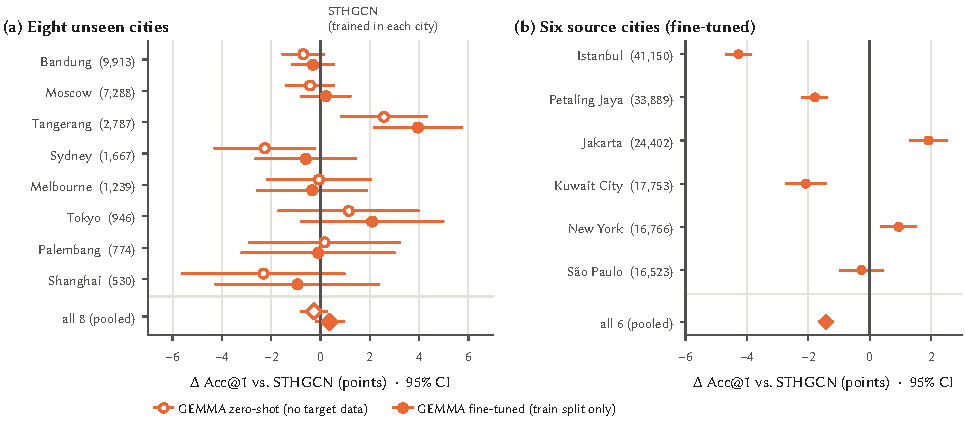
\includegraphics[width=\textwidth]{fig3_main_forest.pdf}
\caption{\textbf{Per-city difference to STHGCN} (Acc@1 points, 95\% CI from test sampling and seed spread; number of
test queries in brackets). (a)~On unseen cities, zero-shot \gemma{} (hollow) is statistically indistinguishable
from STHGCN in 6 of 8 cities (better in Tangerang, worse in Sydney); fine-tuned \gemma{} (solid) is
indistinguishable in 7 and significantly better in Tangerang, with no significant loss. (b)~On the six source cities STHGCN keeps an in-domain advantage in Istanbul, Petaling Jaya and
Kuwait City; \gemma{} is better in Jakarta and New York.}
\label{fig:forest}
\end{figure*}

% ---------------------------------------------------------------- Figure 4
\begin{figure}[t]
\centering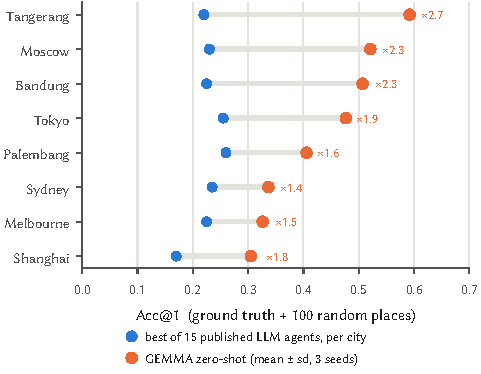
\includegraphics[width=\columnwidth]{fig4_llm.pdf}
\caption{\textbf{Zero-shot \gemma{} vs.\ LLM agents} under the LLM-Move protocol. Blue: the best of the 15 published
LLM agents in each city (an oracle choice of framework and model); orange: \gemma{} (3 seeds), which runs no LLM.}
\label{fig:llm}
\end{figure}

% ---------------------------------------------------------------- Figure 5
\begin{figure*}[t]
\centering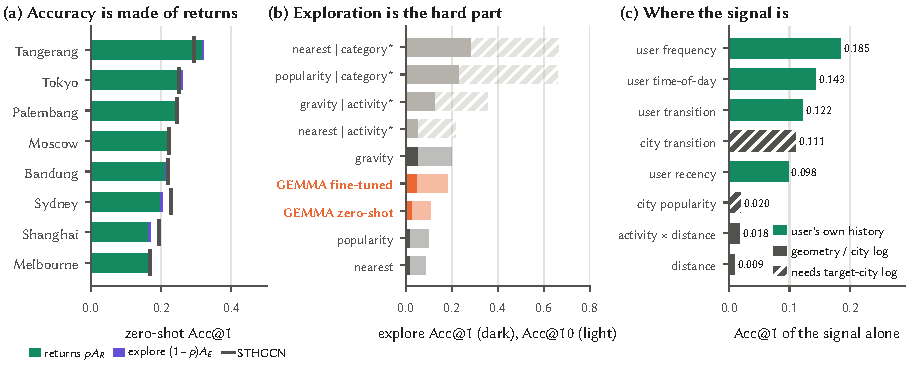
\includegraphics[width=\textwidth]{fig5_anatomy.pdf}
\caption{\textbf{Anatomy of the prediction.} (a)~Zero-shot Acc@1 split into returns ($\rho A_R$) and explorations
($(1-\rho)A_E$); almost all hits are returns. (b)~Ranking a \emph{new} place, given that the user explores (mean over the
8 unseen cities): \gemma{} beats distance and popularity rankers, but oracles that know the true activity or category
(*, hatched) show how much remains. (c)~Single signals ranked alone: the user's own frequency, time-of-day and
transitions carry most of the information; hatched signals need a log of the target city.}
\label{fig:anatomy}
\end{figure*}

% ---------------------------------------------------------------- Figure 6
\begin{figure*}[t]
\centering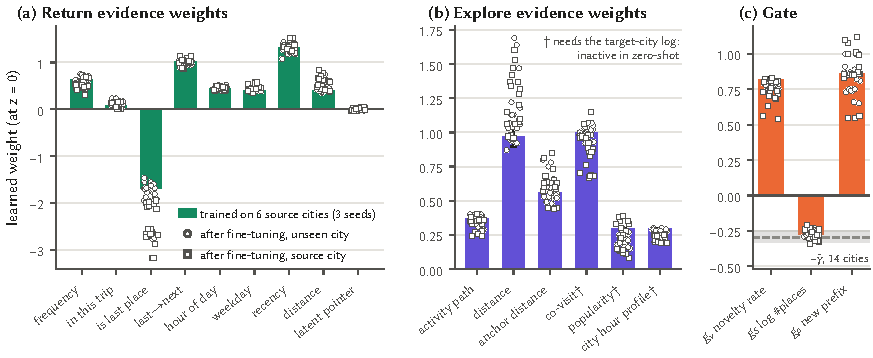
\includegraphics[width=\textwidth]{fig6_weights.pdf}
\caption{\textbf{Learned parameters.} Bars: values learned on the six source cities (mean $\pm$ sd over 3 seeds).
Markers: values after fine-tuning in each unseen (circles) or source (squares) city. Fine-tuning changes the return
weights by a median of 8\% (relative $L_1$); only the largest cities move further, mostly through the is-last
penalty. (c)~The gate's coefficient on $\log S_u$ falls inside the range of $-\gamma$ measured in the
14 evaluated cities (grey band: inter-quartile range).}
\label{fig:weights}
\end{figure*}

% ---------------------------------------------------------------- Figure 7
\begin{figure}[t]
\centering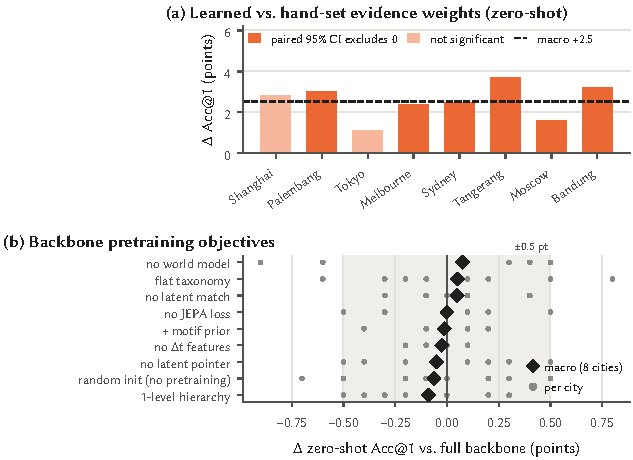
\includegraphics[width=\columnwidth]{fig7_ablation.pdf}
\caption{\textbf{Ablations (zero-shot).} (a)~Learning the evidence weights on source cities instead of setting them by
hand adds 2.5 points (macro over 8 unseen cities). (b)~Removing representation-learning objectives from the backbone
changes accuracy by less than 0.1 point on average: the transfer does not come from pretraining the encoder.}
\label{fig:ablation}
\end{figure}

% ---------------------------------------------------------------- Figure 8
\begin{figure}[t]
\centering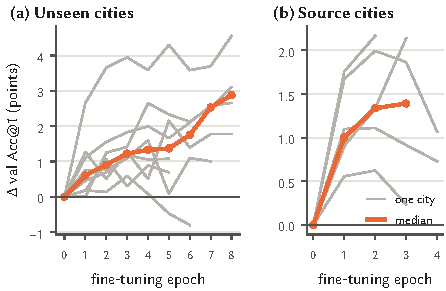
\includegraphics[width=\columnwidth]{fig8_finetune.pdf}
\caption{\textbf{Fine-tuning dynamics.} Validation Acc@1 relative to the transferred model (epoch 0). Gains are
small and arrive within the first epochs.}
\label{fig:finetune}
\end{figure}

\begin{table}[t]
\caption{Aggregate results on the eight unseen cities. Fine-tuned GEMMA is shown with the test-time
history drawn from the training split only (as STHGCN) and from train+validation.}
\label{tab:aggregate}
\small\setlength{\tabcolsep}{4pt}
\begin{tabular}{lccc}
\toprule
 & \multicolumn{2}{c}{Acc@1} & NDCG@5 \\
\cmidrule(lr){2-3}\cmidrule(lr){4-4}
Model & macro & pooled & macro \\
\midrule
GETNext & 0.1640 & 0.1771 & 0.2431 \\
STHGCN & 0.2274 & 0.2278 & 0.3149 \\
\midrule
GEMMA zero-shot & 0.2250 & 0.2252 & 0.3200 \\
GEMMA FT (train) & 0.2324 & 0.2316 & 0.3330 \\
GEMMA FT (train+val) & 0.2348 & 0.2334 & 0.3359 \\
\bottomrule
\end{tabular}
\end{table}

\begin{table}[t]
\caption{Ablations: change of zero-shot macro Acc@1 (points, eight unseen cities).}
\label{tab:ablation}
\small
\begin{tabular}{lr}
\toprule
Variant & $\Delta$Acc@1 \\
\midrule
Learned evidence weights $\to$ hand-set & -2.5 \\
no world-model objective & +0.1 \\
no JEPA objective & +0.0 \\
no backbone pretraining & -0.1 \\
flat activity taxonomy & +0.1 \\
no latent pointer & -0.1 \\
\bottomrule
\end{tabular}
\end{table}

\begin{table}[t]
\caption{Learned parameters (at $\mathbf{z}=0$). Source: trained on six cities, mean $\pm$ sd over 3 seeds.
Fine-tuned: range over the eight unseen cities $\times$ 3 seeds after fine-tuning. $^\dagger$\,needs the target-city log,
inactive in zero-shot.}
\label{tab:weights}
\small\setlength{\tabcolsep}{4pt}
\begin{tabular}{lcc}
\toprule
Parameter & Source-trained & Fine-tuned (range) \\
\midrule
\multicolumn{3}{l}{\textit{Return evidence $\mathbf{w}_0$}} \\
frequency & 0.63 $\pm$ 0.04 & 0.46 -- 0.75 \\
in this trip & 0.07 $\pm$ 0.03 & 0.04 -- 0.23 \\
is last place & -1.69 $\pm$ 0.02 & -2.78 -- -1.47 \\
last$\to$next & 1.02 $\pm$ 0.02 & 0.89 -- 1.07 \\
hour of day & 0.44 $\pm$ 0.01 & 0.39 -- 0.52 \\
weekday & 0.41 $\pm$ 0.01 & 0.36 -- 0.46 \\
recency & 1.32 $\pm$ 0.05 & 1.07 -- 1.46 \\
distance & 0.39 $\pm$ 0.03 & 0.35 -- 0.74 \\
latent pointer & -0.01 $\pm$ 0.01 & -0.04 -- 0.04 \\
\midrule
\multicolumn{3}{l}{\textit{Explore evidence $\mathbf{w}'_0$}} \\
activity path & 0.37 $\pm$ 0.01 & 0.28 -- 0.40 \\
distance & 0.97 $\pm$ 0.08 & 0.87 -- 1.69 \\
anchor distance & 0.56 $\pm$ 0.01 & 0.48 -- 0.80 \\
co-visit$^\dagger$ & 1.00 $\pm$ 0.00 & 0.92 -- 1.07 \\
popularity$^\dagger$ & 0.30 $\pm$ 0.00 & 0.13 -- 0.27 \\
city hour profile$^\dagger$ & 0.30 $\pm$ 0.00 & 0.19 -- 0.30 \\
\midrule
\multicolumn{3}{l}{\textit{Gate}} \\
$g_\nu$ novelty rate & 0.82 $\pm$ 0.01 & 0.73 -- 0.81 \\
$g_S$ log \#places & -0.27 $\pm$ 0.01 & -0.30 -- -0.23 \\
$g_p$ new prefix & 0.86 $\pm$ 0.02 & 0.65 -- 1.00 \\
\bottomrule
\end{tabular}
\end{table}


\IfFileExists{../out/figs/fig9_evidence_ablation.pdf}{
\begin{figure}[t]\centering\includegraphics[width=\columnwidth]{fig9_evidence_ablation.pdf}
\caption{\textbf{Leave-one-evidence-out and gate ablations} (zero-shot, test time, 3 seeds).}\end{figure}}{}
\IfFileExists{../out/figs/fig10_history.pdf}{
\begin{figure}[t]\centering\includegraphics[width=\columnwidth]{fig10_history.pdf}
\caption{\textbf{Cold start.} Zero-shot Acc@1 when only the $k$ most recent check-ins of each user are visible.}\end{figure}}{}
\end{document}
